\documentclass[a4paper]{article}
\usepackage[utf8x]{inputenc}
\usepackage[T1,T2A]{fontenc}
\usepackage[russian]{babel}
\usepackage{hyperref}
\usepackage{indentfirst}
\usepackage{listings}
\usepackage{color}
\usepackage{here}
\usepackage{array}
\usepackage{multirow}
\usepackage{graphicx}
\usepackage{amsmath} 
\usepackage{spverbatim}

\usepackage{caption}
\renewcommand{\lstlistingname}{Программа} % заголовок листингов кода

\lstset{ %
	extendedchars=\true,
	keepspaces=true,
	language=bash,					% choose the language of the code
	basicstyle=\footnotesize,		% the size of the fonts that are used for the code
	numbers=left,					% where to put the line-numbers
	numberstyle=\footnotesize,		% the size of the fonts that are used for the line-numbers
	stepnumber=1,					% the step between two line-numbers. If it is 1 each line will be numbered
	numbersep=5pt,					% how far the line-numbers are from the code
	backgroundcolor=\color{white},	% choose the background color. You must add \usepackage{color}
	showspaces=false				% show spaces adding particular underscores
	showstringspaces=false,			% underline spaces within strings
	showtabs=false,					% show tabs within strings adding particular underscores
	frame=single,           		% adds a frame around the code
	tabsize=2,						% sets default tabsize to 2 spaces
	captionpos=b,					% sets the caption-position to bottom
	breaklines=true,				% sets automatic line breaking
	breakatwhitespace=false,		% sets if automatic breaks should only happen at whitespace
	escapeinside={\%*}{*)},			% if you want to add a comment within your code
	postbreak=\raisebox{0ex}[0ex][0ex]{\ensuremath{\color{red}\hookrightarrow\space}}
}

\usepackage[left=2cm,right=2cm,
top=2cm,bottom=2cm,bindingoffset=0cm]{geometry}
\renewcommand{\labelitemi}{$\diamond$}
\begin{document}	% начало документа

\begin{titlepage}	% начало титульной страницы

	\begin{center}		% выравнивание по центру

		\largeФедеральное государственное автономное образовательное учреждение высшего образования «Санкт-Петербургский политехнический университет Петра Великого» \\
		\large Институт компьютерных наук и технологий \\
		\large Кафедра компьютерных систем и программных технологий\\[2cm]
		% название института, затем отступ 6см
		
	    \vfill
		\hugeТелекоммуникационные технологии\\[0.5cm] % название работы, затем отступ 0,5см
		\large Лабораторная работа №5:\\
		Частотная и фазовая модуляция\\[4.8cm]

	\end{center}

	\begin{flushright} % выравнивание по правому краю
		\begin{minipage}{0.25\textwidth} % врезка в половину ширины текста
			\begin{flushleft} % выровнять её содержимое по левому краю

				\large\textbf{Работу выполнил:}\\
				\large Сергеев ~А.А.\\
				\large {Группа:} 33531/2\\
				
				\large \textbf{Преподаватель:}\\
				\large Богач ~Н.В.\\

			\end{flushleft}
		\end{minipage}
	\end{flushright}
	
	\vfill % заполнить всё доступное ниже пространство

	\begin{center}
	\large Санкт-Петербург\\
	\large \the\year % вывести дату
	\end{center} % закончить выравнивание по центру

\thispagestyle{empty} % не нумеровать страницу
\end{titlepage} % конец титульной страницы
\vfill % заполнить всё доступное ниже пространство

% Содержание
\tableofcontents
\newpage
\section{Цель}
Изучение частотной и фазовой модуляции/демодуляции сигнала.
\section{Постановка задачи}
\begin{enumerate}
    \item Сгенерировать однотональный сигнал низкой частоты.
    \item Выполнить фазовую модуляцию/демодуляцию сигнала по закону $u(t)=(U_m\cos{(\Omega t+ks(t))})$, используя встроенные функции $MatLab$ $pmmod$, $pmdemod$.
    \item Получить спектр модулированного сигнала.
    \item Выполнить частотную модуляцию/демодуляцию по закону $u(t)=U_m cos(\omega_0 t+k\int_{0}^{t}s(t)dt+\phi_0)$, используя встроенные функции $MatLab$ $fmmod$, $fmdemod$.
\end{enumerate}

\section{Теоретический раздел}
Как правило, информационные сигналы являются низкочастотными и ограниченными по ширине спектра, тогда как методы передачи сигналов рассчитаны на работу с высокочастотным сигналом. Перенос спектра сигналов из низкочастотной области на заданную частоту, т.е. в выделенную для их передачи область высоких частот выполняется операцией модуляции.\\
$s(t)$ -- низкочастотный сигнал, подлежащий передаче по какому-либо каналу связи. В канале связи для передачи данного сигнала выделяется определенный диапазон высоких частот и формируется вспомогательный периодический высокочастотный сигнал $u(t) = f(t; a_1, a_2, ... a_m).$ Совокупность параметров $a_i$ определяет форму вспомогательного сигнала. Значения параметров $a_i$ в отсутствие модуляции являются величинами постоянными.\\
Если на один из этих параметров перенести сигнал $s(t)$, т.е. сделать его значение пропорционально зависимым от значения $s(t)$ во времени (или по любой другой независимой переменной), то форма сигнала $u(t)$ приобретает новое свойство. Она служит для переноса информации, содержащейся в сигнале $s(t)$. Сигнал $u(t)$ называется несущим сигналом, несущим колебанием или просто несущей, а физический процесс переноса информации на параметры несущего сигнала -- его модуляцией. Исходный информационный сигнал $s(t)$ называют модулирующим, результат модуляции -- модулированным сигналом. Обратную операцию выделения модулирующего сигнала из модулированного колебания называют демодуляцией или детектированием.\\
Наиболее распространенной формой несущих сигналов являются гармонические колебания $u(t)=Ucos(\omega t+\phi)$, которые имеют три свободных параметра: $U$, $\omega$ и $\phi$. В зависимости от того, на какой из данных параметров переносится информация, различают амплитудную (АМ), частотную (ЧМ) или фазовую (ФМ) модуляцию несущего сигнала.\\
При использовании в качестве несущих сигналов периодических последовательностей импульсов (например, прямоугольных) свободными параметрами модуляции могут быть амплитуда, длительность, частота следования и фаза (положение импульса относительно тактовой точки) импульсов. Таким образом, существует три основных вида импульсной модуляции: АИМ, ЧИМ и ФИМ.
\subsection{Фазовая модуляция}
При фазовой модуляции значение фазового угла постоянной несущей частоты колебаний $\omega_0$ пропорционально амплитуде модулирующего сигнала $s(t)$. Соответственно, уравнение ФМ-сигнала определяется выражением:
$$u(t) = U_m cos[\omega_0 t+k*s(t)],$$ где $k$ -- коэфициент пропорциональности.

При $s(t) = 0$, ФМ-сигнал является простым гармоническим колебанием. С увеличением значений $s(t)$ полная фаза колебаний $\verphi(t)=\omega_0t + k*s(t)$ нарастает во времени быстрее и опережает линейное нарастание $\omega_0 t$. Соответственно, при уменьшении значений $s(t)$ скорость роста полной фазы во времени спадает. В моменты экстремальных значений $s(t)$ абсолютное значение фазового сдвига $\delta \verphi $между ФМ-сигналом и значением $\omega t$ немодулированного колебания также является максимальным и носит название девиации фазы (вверх $\delta\phi_{B}=k*s_{max}(t)$, или вниз $\delta \phi_{h} = k*s_{min}(t)$ с учетом знака экстремальных значений модулирующего сигнала).
\subsection{Частотная модуляция}
Частотная модуляция характеризуется линейной связью модулирующего сигнала с мгновенной частотой колебаний, при которой мгновенная частота колебаний образуется сложением частоты высокочастотного несущего колебания $\omega_0$ со значением амплитуды модулирующего сигнала с определенным коэффициентом пропорциональности $k$: $$\omega(t)=\omega_0 +k*s(t).$$
Соответственно, полная фаза колебаний:
$$\verphi(t)=\omega_0(t) + k \int_{-\infty}^t s(t)dt или \verphi(t)=\omega_0(t) + k \int_{-\infty}^t s(t)dt +\phi_0$$
Уравнение ЧМ-сигнала:
$$u(t)=U_m cos(\omega_0(t)+k\int_0^t s(t)dt +\phi_0)$$
Аналогично ФМ, для характеристики глубины частотной модуляции используются понятия девиации частоты вверх:
 $\delta \omega_{B} = k*s_{max}(t)$
 и вниз $\delta \omega_{h} = k*s_{min}(t)$
\section{Ход работы}
\subsection{Фазовая модуляция}
\lstinputlisting[language=Matlab]{lab5/phase_modulation.m}\\
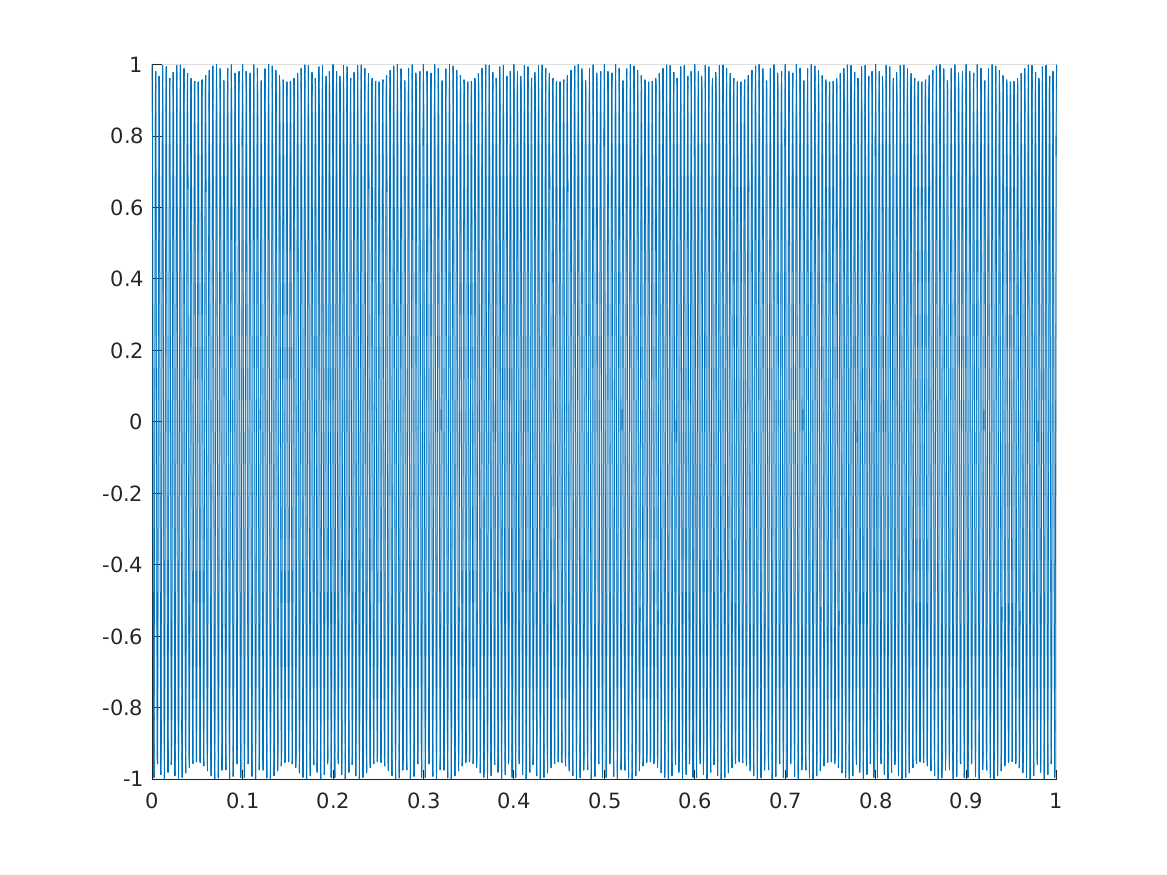
\includegraphics[scale=0.7]{lab5/figures/figure_1.png}\\
И её спектр:\\
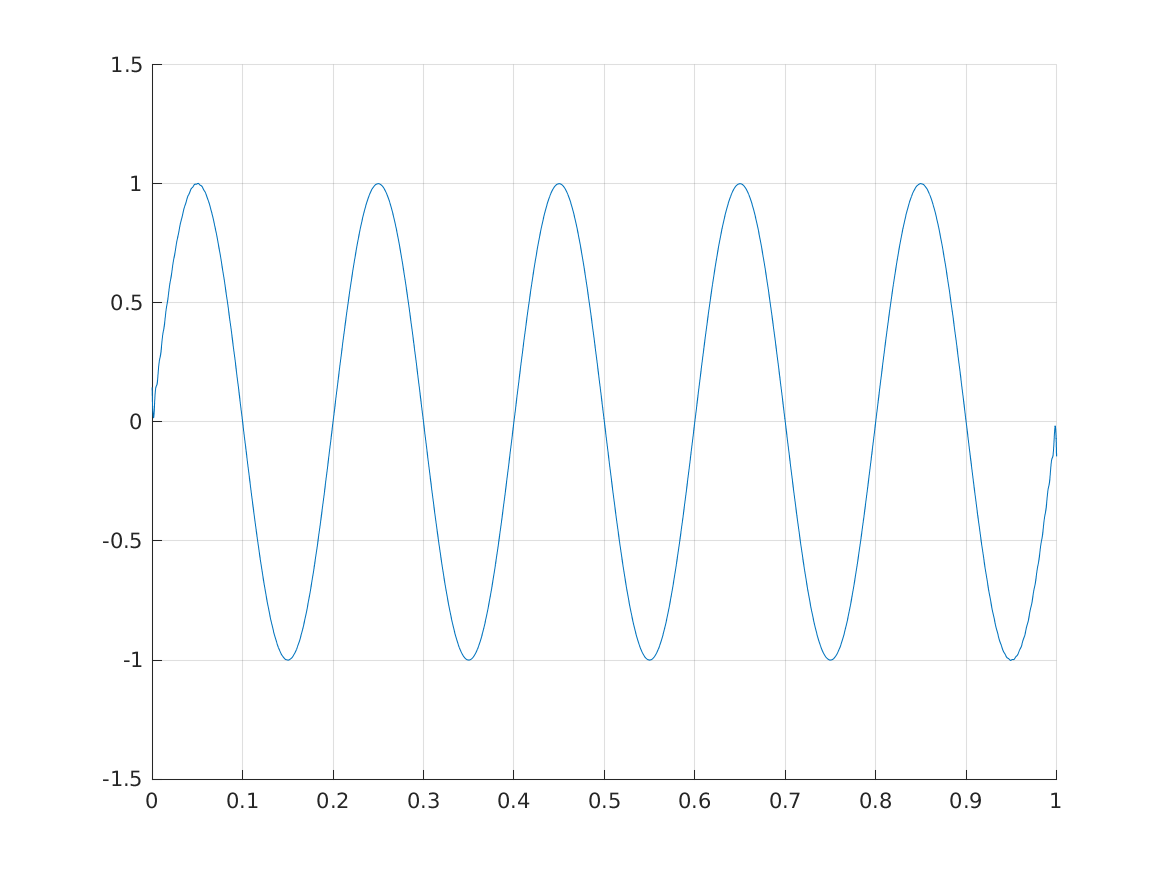
\includegraphics[scale=0.7]{lab5/figures/figure_2.png}\\
\newpage
Проведем демодуляцию:
\lstinputlisting[language=Matlab]{lab5/demodulation.m}\\
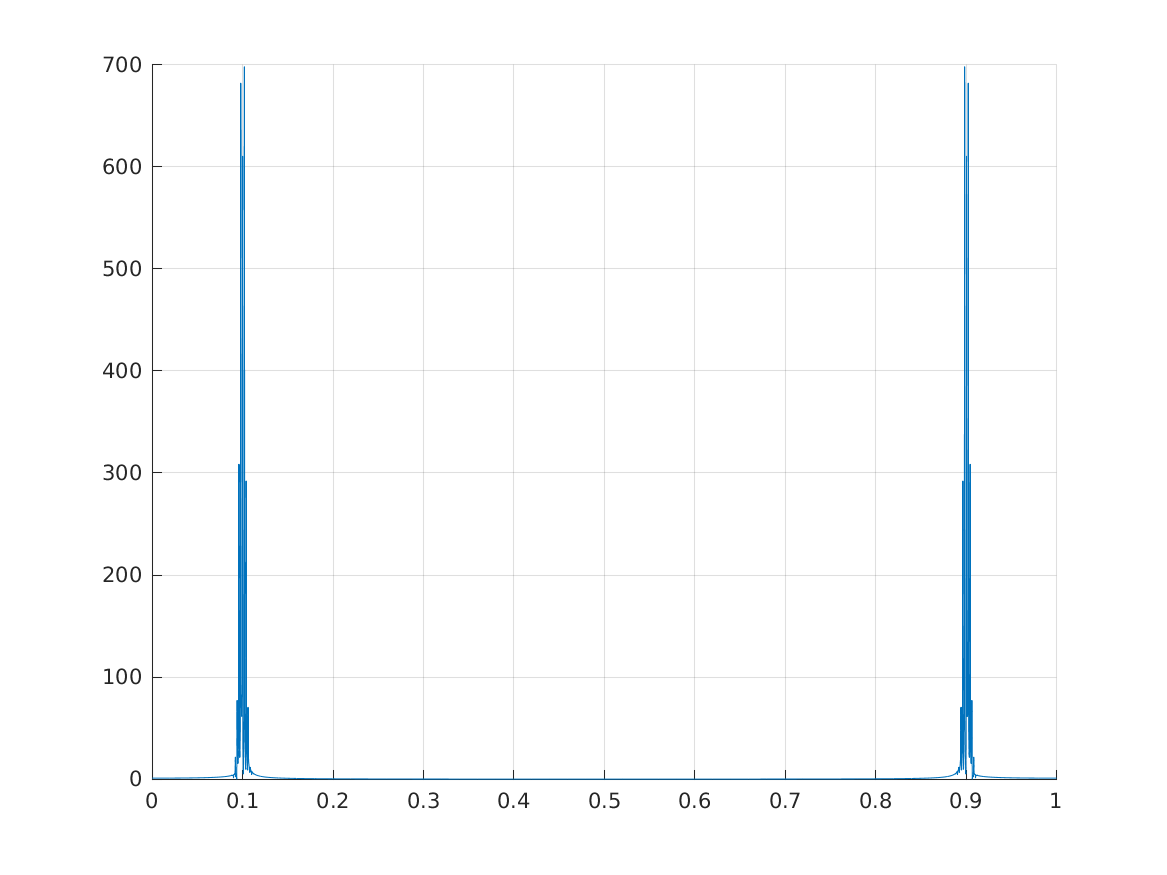
\includegraphics[scale=0.7]{lab5/figures/figure_3.png}\\
\subsection{Частотная модуляция}
Находим частотную модуляцию построенного сигнала:
\lstinputlisting[language=Matlab]{lab5/frequency_modulation.m}\\
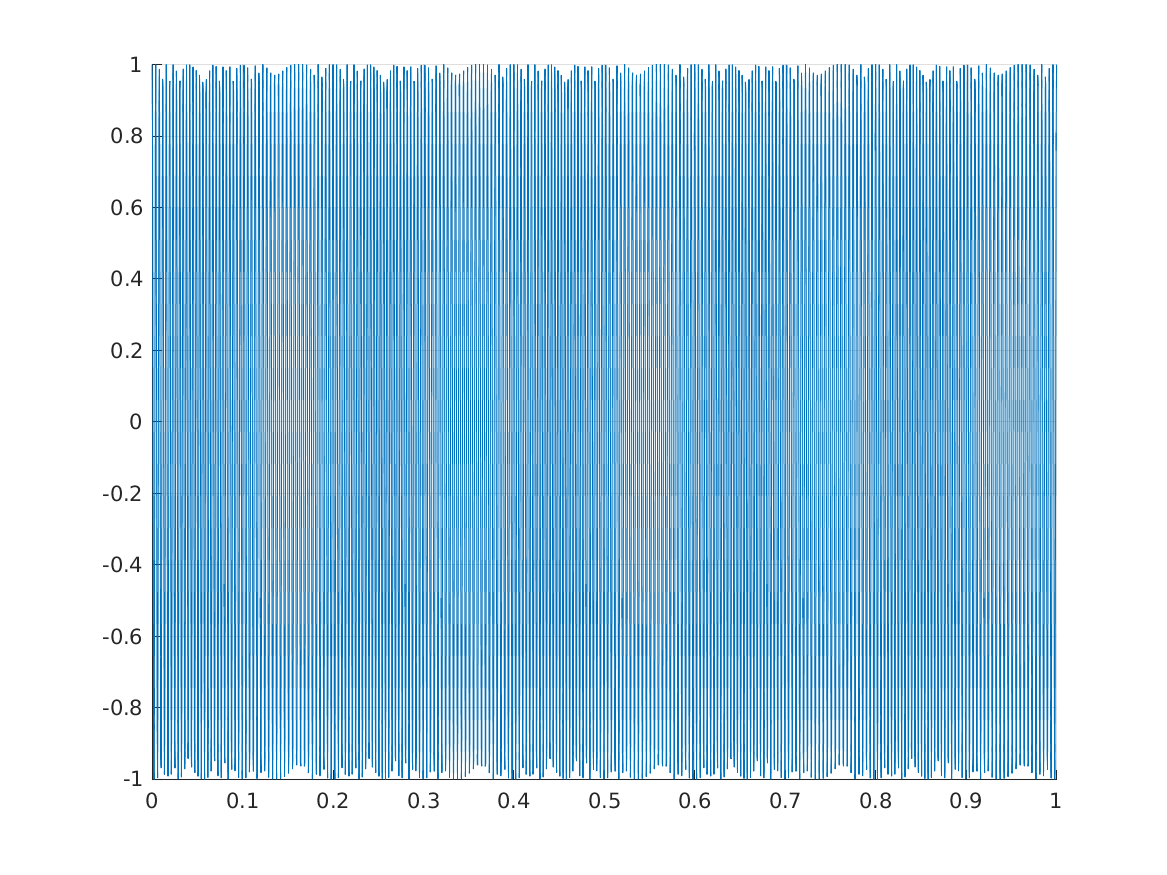
\includegraphics[scale=0.7]{lab5/figures/figure_4.png}\\
И её спектр:\\
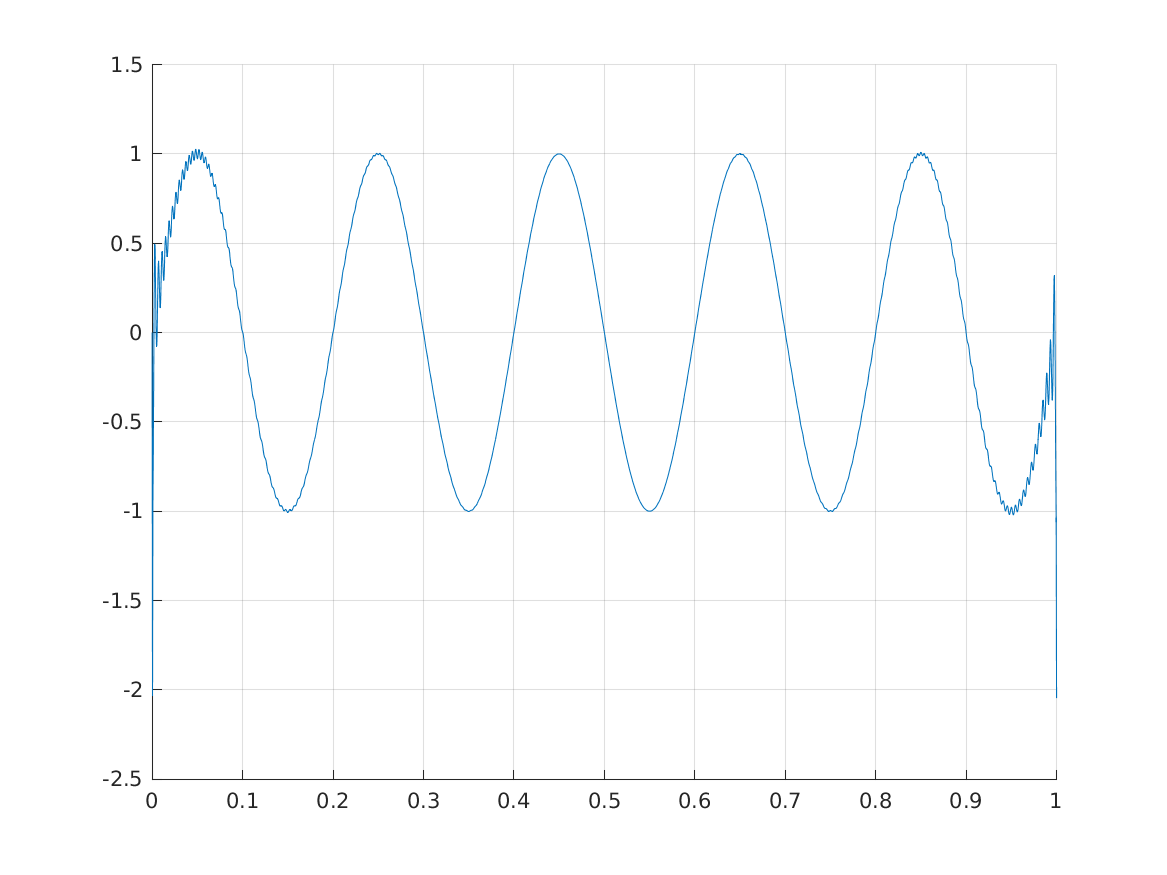
\includegraphics[scale=0.7]{lab5/figures/figure_5.png}\\
Проведем демодуляцию:
\lstinputlisting[language=Matlab]{lab5/demodulation.m}\\
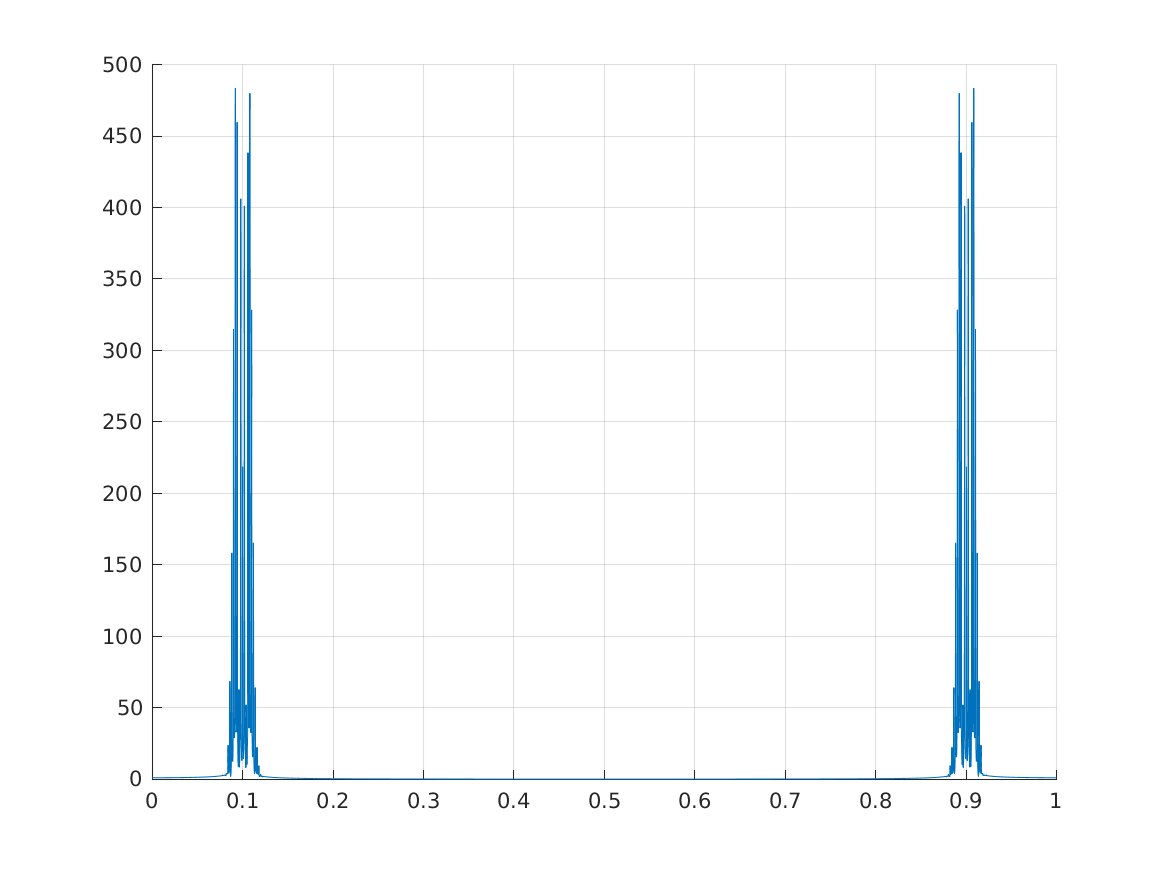
\includegraphics[scale=0.7]{lab5/figures/figure_6.png}\\
Демодулируемый сигнал совпал с исходным\\
\section{Вывод}
Таким образом, достоинством частотной модуляции являются высокая помехоустойчивость,
более эффективное использование мощности передатчика, а также
сравнительная простота получения модулированных сигналов.\\
Основным недостатком данной модуляции является большая ширина спектра модулированного сигнала.\\
Частотная модуляция используется в системах телевизионного вещания (для передачи сигналов звукового сопровождения), системах спутникового теле- и радиовещания, системах высококачественного стереофонического вещания (FM диапазон), радиорелейных линиях (РРЛ), сотовой телефонной связи.\\

Достоинствами фазовой модуляции являются высокая помехоустойчивость и более эффективное использование мощности передатчика.\\
Недостатками фазовой модуляции являются большая ширина спектра, сравнительная трудность получения модулированных сигналов и их детектирование.
\end{document}